\documentclass[border=5mm]{standalone}
\usepackage{tikz}

\begin{document}

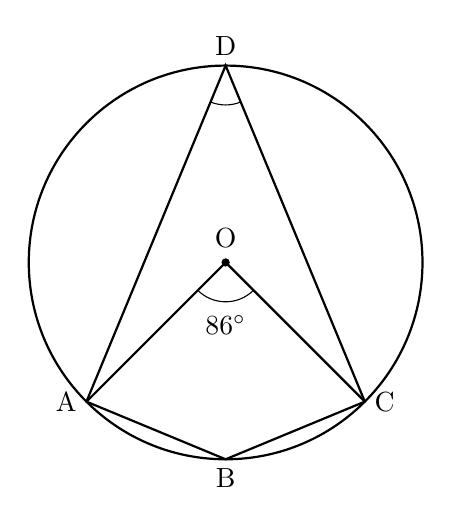
\begin{tikzpicture}[scale=1]

% 1. Draw the main circle with center O
\draw[thick] (0,0) circle (2.5cm);
\fill (0,0) circle (1.5pt) node[above=2pt] {O};

% 2. Define coordinates for points (approximate to image)
\coordinate (D) at (90:2.5);
\coordinate (A) at (225:2.5);
\coordinate (B) at (270:2.5);
\coordinate (C) at (315:2.5);

% 3. Draw the segments for the inscribed and central angles
\draw[thick] (A) -- (D) -- (C); % Angle at D
\draw[thick] (A) -- (0,0) -- (C); % Angle at O
\draw[thick] (A) -- (B) -- (C); % Segments at B

% 4. Label the points
\node[above] at (D) {D};
\node[left] at (A) {A};
\node[below] at (B) {B};
\node[right] at (C) {C};

% 5. Draw the angle arc at O (Central Angle)
\draw (225:0.5) arc (225:315:0.5);
\node at (270:0.8) {$86^{\circ}$};

% 6. Draw the angle arc at D (Inscribed Angle)
% This creates a clear arc centered at point D
\begin{scope}
    \clip (D) -- (A) -- (C) -- cycle;
    \draw (D) circle (0.5cm);
\end{scope}

\end{tikzpicture}

\end{document}
